\documentclass[12pt,a4paper]{report}
\usepackage[none]{hyphenat}
\usepackage{setspace}
\usepackage[left=3.7cm,right=2.5cm,top=2.5cm,bottom=2.5cm]{geometry}
\usepackage{amsmath}
\usepackage{url}
\usepackage{graphicx}
\usepackage{float}
\usepackage[toc,page]{appendix}
\usepackage{multirow}
\usepackage{titling}
\usepackage[acronym]{glossaries}
\usepackage{subcaption}
\usepackage{array}
\usepackage{dirtytalk}

\usepackage{listings}
% \usepackage{showframe}

% Default fixed font does not support bold face
\DeclareFixedFont{\ttb}{T1}{txtt}{bx}{n}{11} % for bold
\DeclareFixedFont{\ttm}{T1}{txtt}{m}{n}{11}  % for normal

% Custom colors
\usepackage{color}
\definecolor{deepblue}{rgb}{0,0,0.5}
\definecolor{deepred}{rgb}{0.6,0,0}
\definecolor{deepgreen}{rgb}{0,0.5,0}
\definecolor{deepgrey}{rgb}{0.329, 0.431, 0.478}

% Python style for highlighting
\newcommand\pythonstyle{\lstset{
    language=Python,
    basicstyle=\tiny\ttm,
    otherkeywords={self},            
    keywordstyle=\ttb\color{deepblue},
    emph={MyClass,__init__},          % Custom highlighting
    emphstyle=\ttb\color{deepred},    % Custom highlighting style
    stringstyle=\ttm\color{deepgreen},
    commentstyle=\ttm\color{deepgrey},
    frame=tb,                        
    showstringspaces=false,          
    breaklines=true,
    postbreak=\mbox{\textcolor{red}{$\hookrightarrow$}\space},
}}


% Python environment
\lstnewenvironment{python}[1][]
{
    \pythonstyle
    \lstset{#1}
}{}

% Python for external files
\newcommand\pythonexternal[2][]{{
\pythonstyle
\lstinputlisting[#1]{#2}}}

% Python for inline
\newcommand\pythoninline[1]{{\pythonstyle\lstinline!#1!}}


\author{P.B.W. Amaradiwakara}

\linespread{2}
\graphicspath{ {images/} }

\begin{document}
\newacronym{stft}{STFT}{Short Time Fourier Transformation}
\newacronym{sift}{SIFT}{Scale Invarient Feature Transform}
\newacronym{dog}{DoG}{Difference of Gaussians}

\begin{titlepage}
    \begin{center}

        
\includegraphics[width=3cm]{uoc.png}\\
        \vspace{24pt}
        \textbf{\Huge{Blockchain-based Digital Identity to Reduce Duplicate Identity Verification}}


        \vspace{36pt}
        \textbf{{\Large{P.B.W. Amaradiwakara}}}\\
        \textbf{{\Large{Index No : 15000087}}}\\

        \vspace{36pt}
        \textbf{{\Large{Supervisor : Dr. Kasun De Zoysa}}}\\
        \textbf{{\Large{Co-supervisor : Dr. M.D.J.S. Goonetillake}}}\\

        \vspace{60pt}
        \textbf{{\Large{February 2020}}}\\
        
        \vspace{12pt}
        \singlespacing
        \large {Submitted in partial fulfillment of the requirements of the}\\
        \large {B.Sc in Computer Science Final Year Project (SCS4124)}
        
        \vspace{24pt}
        
\includegraphics[width=3.5cm	]{Ucsc.jpg}\\

    \end{center}
\end{titlepage}
\clearpage

\linespread{2}
\begin{titlepage}
    \begin{center}
        \textbf{\Huge{Protecting Copyright Ownership via Identification of Remastered Music in Radio Broadcasts}}
        \vfill
        \huge{P.B.W. Amaradiwakara}
    \end{center}
\end{titlepage}

\pagenumbering{roman}
\onehalfspacing
\sloppy
\chapter*{Declaration}
\addcontentsline{toc}{chapter}{Declaration}

I certify that this dissertation does not incorporate, without acknowledgement, any material previously submitted for a degree or diploma in any university and to the best of my knowledge and belief, it does not contain any material previously published or written by another person or myself except where due reference is made in the text. I also hereby give consent for my dissertation, if accepted, be made available for photocopying and for interlibrary loans, and for the title and abstract to be made available to outside organizations.

\vspace{0.5cm}
\noindent
Candidate Name : P.B.W. Amaradiwakara

\vspace{1.25cm}
\noindent
\makebox[130pt]{\dotfill} \\
Signature of Candidate \hspace{144pt} Date :


\vspace{1cm}
\noindent
This is to certify that this dissertation is based on the work of

\vspace{6pt}
\noindent
Mr. P.B.W. Amaradiwakara

\vspace{6pt}
\noindent
under my supervision. The thesis has been prepared according to the format stipulated and is of acceptable standard.

\vspace{0.5cm}
\noindent
Supervisor Name : Dr. Kasun De Zoysa

\vspace{1cm}
\noindent
\makebox[130pt]{\dotfill} \\
Signature of Supervisor \hspace{144pt} Date :

\vspace{1cm}
\noindent
Co-supervisor Name : Dr. M.D.J.S. Goonetillake

\vspace{1cm}
\noindent
\makebox[130pt]{\dotfill} \\
Signature of Co-supervisor \hspace{128pt} Date :


\chapter*{Abstract}
\addcontentsline{toc}{chapter}{Abstract}



\chapter*{Preface}
\addcontentsline{toc}{chapter}{Preface}

\chapter*{Acknowledgement}
\addcontentsline{toc}{chapter}{Acknowledgement}



\renewcommand\contentsname{Table of Contents\\}
\tableofcontents
\clearpage

\pagenumbering{arabic}

%introduction Chapter
\chapter{Introduction}
\section{Background to the Research}
\vspace{12pt}


Sri Lankan government is still using lots of manual processes for identity verification of people. 
People have to keep providing their legal documents in order to work with the authority. There are 
several basic legal documents like “Birth Certificate”, “National Identity Card”, “Driving License”, 
“Passport”  for a person in Sri Lanka. And also have other qualification certificates like “ University 
Transcript”, “School Leaving Certificate”, “Character Certificate” and more. The current process is, 
people have to provide their information in a legal manner and claim their assertions. When they need 
to interact with the authority, they should provide the same information or assertions over again. 
The problem in this context is people provide their very same information or assertions on different 
authority sectors and organizations. This is a major problem when considering the government sectors. 
Since there are millions of people in a country, a government needs a provable claim to identify and 
verify people. 

\vspace{12pt}


Official evidence of identity is basic to a person's capacity to implement their privileges and secure 
access to a wide scope of essential administrations, for example, medicinal services, training, portable 
availability, social assurances, and budgetary administrations. Sri Lanka has essential and practical 
personality frameworks that are very much evolved and hearty. Responsibility for National Identity Card 
(NIC) is high, revealed at 95 percent for men and 90 percent for ladies, with just little pockets of Sri 
Lankan culture more averse to claim a NIC. Birth Certificates and National Identity Cards are major 
identities for verification in Sri Lanka. However, the Birth certificate is a mandatory document for 
claiming the National Identity Card. But most of the time people need to present both NIC and Birth 
certificate. When people need to apply for a Driving license or a university enrollment, again they 
need to present their birth certificate. This is where the duplication of identity verification happens.
 Because of this duplication process, people have to submit their verification documents continuously. 
 And it is more costly and time-wasting criteria. The Sri Lankan government produces more than 300,000 
 birth certificates per year. The birth certificate is the most fundamental identity for identity verification 
 in Sri Lanka.

 \begin{figure}[H]
    \centering
    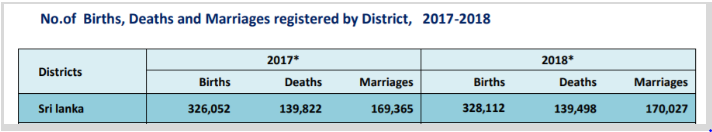
\includegraphics[scale=1]{Capture.png}
    \caption{Sri Lankan Registration certificates}
    \label{fig:threshold}
  \end{figure}

  Birth certificate issued by the Sri Lankan government when birth and every person has it with them. 
  For instance, Pasindu is a civilian in Sri Lanka and has to provide her identity for school applying. 
  Then Pasindu needs to enter a state university and again needs to provide the birth certificate. 
  When Pasindu wants to apply for a driving license, again he needs to present his birth certificate 
  as her identity document. As a solution to this problem, the government can consider a centralized 
  system[1] with a centralized database[2] for identity verification.
  
  \begin{figure}[H]
    \centering
    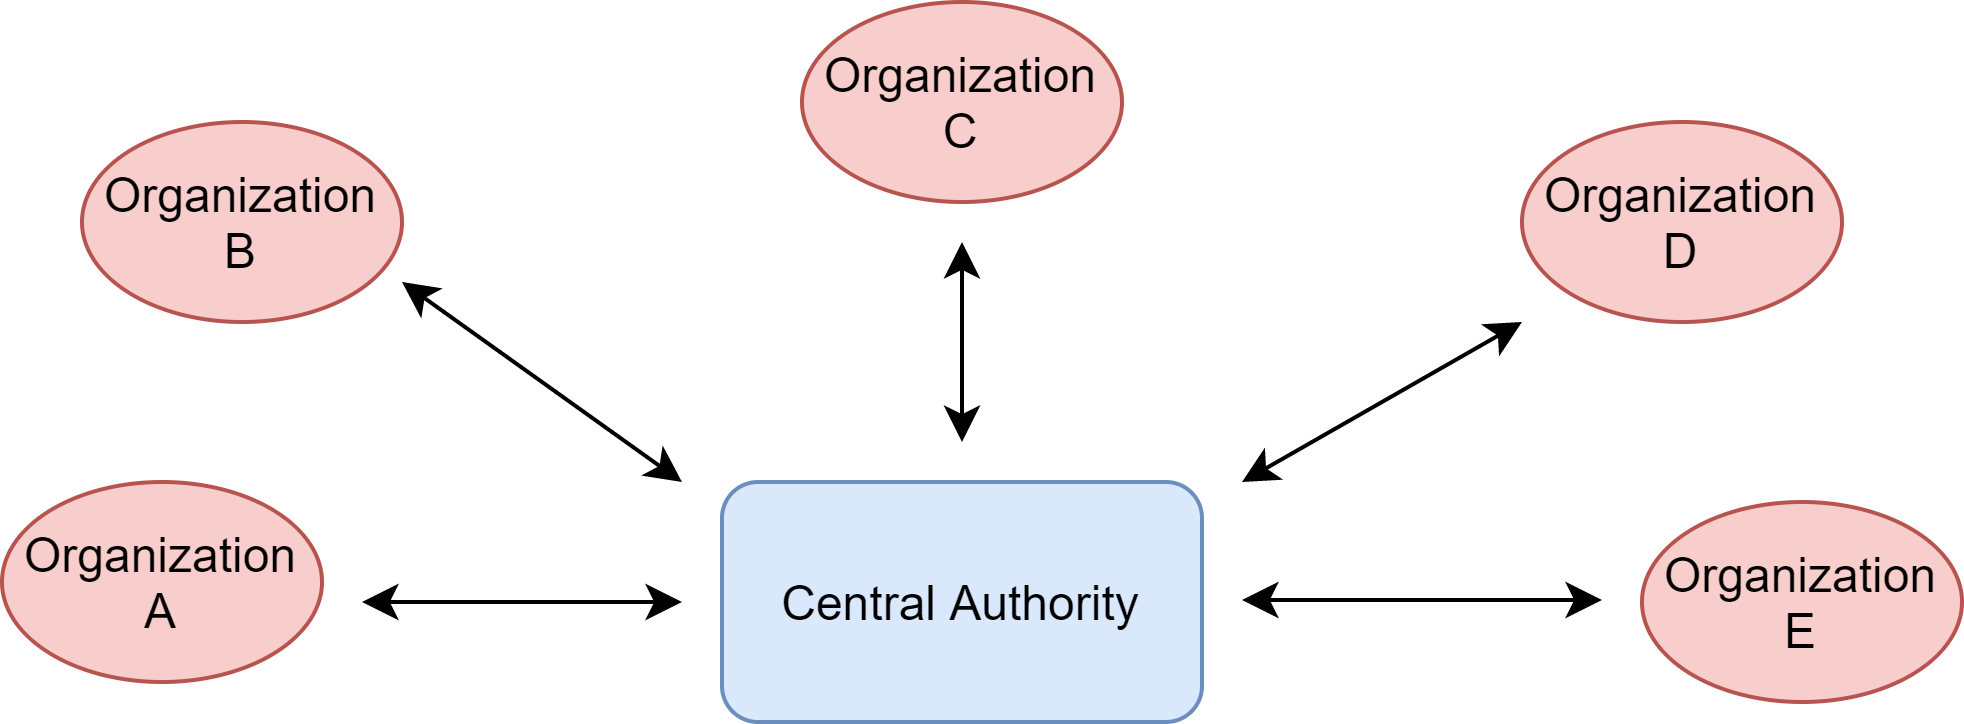
\includegraphics[scale=0.8]{1.png}
    \caption{centralized database}
    \label{fig:threshold}
  \end{figure}

  Centralized systems are systems that use client/server architecture where one or more client nodes 
  are directly connected to a central server. This is the most commonly used type of system in many 
  organizations where the client sends a request to a company server and receives the response. 
  In this centralized system, the government can record the identities of civilians and provide 
  an application program interface (API) for organizations and government sectors that need to 
  verify the identities. Organizations and the government should have a mutual trust for verifying 
  identities. For instance, Alice can verify her claim which could be the birth certificate or any 
  verifiable document with the authority and get an assertion for her claim document. Then Alice 
  can use this assertion when she wants to apply for a driving license. But this centralized 
  system has some limitations and problems.

  \subsection{Limitations}

  \begin{itemize}
    \item It cannot scale up vertically after a certain limit. After this limit, even if it increases 
    the hardware and software capabilities of the server node, the performance will not increase 
    appreciably leading to a cost/benefit ratio < 1.
    \item Bottlenecks can appear when the traffic spikes – as the server can only have a finite number
     of open ports to which can listen to connections from client nodes. So, when high traffic occurs
      like a shopping sale, the server can essentially suffer a Denial-of-Service attack or Distributed
       Denial-of-Service attack.
      
  \end{itemize}

  \subsection{Problems}

  \begin{itemize}
    \item Highly dependent on the network connectivity – System can fail if the nodes lose connectivity as there is only one central node.
    \item No graceful degradation of the system – abrupt failure of the entire system
    \item Less possibility of data backup. If the server node fails and there is no backup, system lose the data straight away
    \item Difficult server maintenance – There is only one server node and due to availability reasons, it is inefficient and unprofessional to take the server down for maintenance. So, updates have to be done on-the-fly(hot updates) which is difficult and the system could break.
    \item Only the government can authorize users.
  \end{itemize}

  To overcome the above limitations and problems, the authority can think of a decentralized solution[3]. 
  In this decentralized system, the government can distribute the centralized database throughout the 
  organizations that are already trusted by the government.

  \begin{figure}[H]
    \centering
    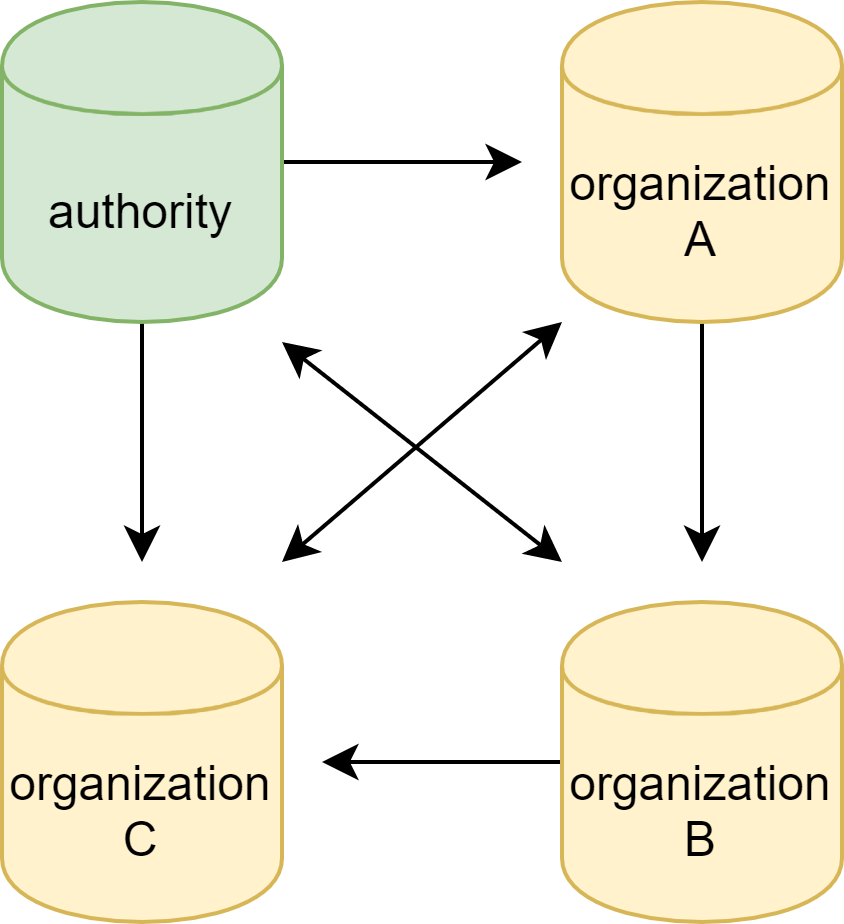
\includegraphics[scale=1]{2.png}
    \caption{decentralized database}
    \label{fig:threshold}
  \end{figure}

  The authority can provide privileges for organizations to verify assertions. But still, the 
  government has the ability to provide privileges and there is no transparency. There are some 
  problems in a system like above to archive the following properties.

  \begin{enumerate}
      \item Existence - Users must have an independent existence.
      \item Control -  Users must control their identities.
      \item Access - Users must have access to their own data.
      \item Transparency - Systems and algorithms must be transparent.
      \item Persistence - Identities must be long-lived.
      \item Portability - Information and services about identity must be transportable
      \item Interoperability - Identities should be as widely usable as possible.
      \item Consent - Users must agree to the use of their identities.
      \item Minimization - Disclosure of claims must be minimized.
      \item Protection - The rights of users must be protected.
  \end{enumerate}

  Authorities cannot archive the above properties using a decentralized database solution. 
  The only possible solution to archive those targets is using blockchain[4] architecture. 
  The blockchain network has no central authority and it is the very definition of a 
  democratized system. Since it is a shared and immutable ledger, the information in it is 
  open for anyone and everyone to see. Hence, anything that is built on the blockchain is 
  by its very nature transparent and everyone involved is accountable for their actions. 
  And it is possible to implement the above properties on top of a blockchain model rather 
  than a decentralized database.


  




\clearpage




\section{Research Problem and Research Questions}

\subsection{Research Questions}
The following questions are founded in this research context. 
\begin{enumerate}
    \item What are the problems of duplicate identity verifications?
    \item How to eliminate the duplicate identity verifications?
    \item Is it technically feasible to implement a block-chain based identity to reduce verifications in a state?
\end{enumerate}

\subsection{Objectives}
The following are objectives in order to archive solutions for the above research questions.
\begin{enumerate}
    \item Find out duplicate identity verifications and problems of duplicating identity verifications.
    \item Solutions for duplicate identity verifications.
    \item Analyzing the feasibility of implementation of the block-chain based identity for a state.
\end{enumerate}

\subsection{Project Aim}
The aim of the research is to utilize computational theories to reduce duplicate identity verifications.


\section{Methodology}

Initially, the current and previous identity management systems have been studied. The first step is to 
digitalize the current identities and make it reliable for identity owners. After a thorough literature 
review, an approach is found: self-sovereign identity. And the next objective is to implement it in the 
real world. and the proposed solution is as follows.

\begin{figure}[H]
    \centering
    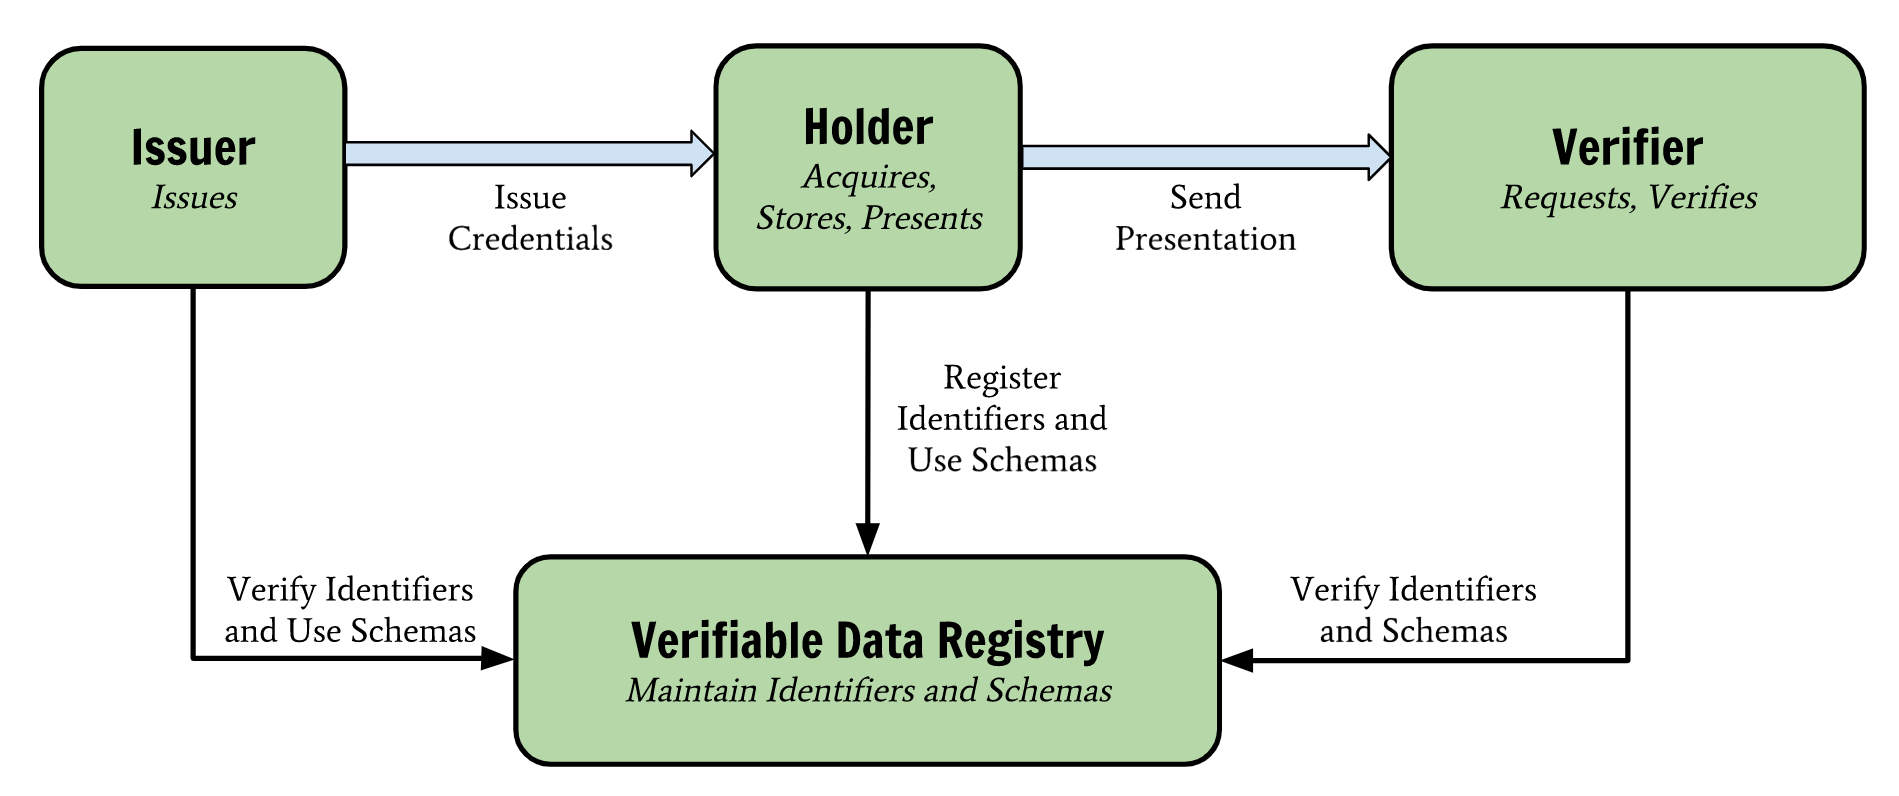
\includegraphics[scale=0.4]{13.png}
    \caption{methodology architecture}
    \label{fig:threshold}
  \end{figure}

  There are 3 main roles in this proposed design.
\begin{enumerate}
    \item Issuer
    \item Holder
    \item Verifier
\end{enumerate}

\begin{itemize}
    \item The holder is the one who wants to verify documents through the system when the holder needs to get credentials for his identity(a legal document or a claim), the issuer should issue the credentials.
    \item Before issuing the credentials, the issuer needs to contact the government or a trust anchor in the system, to get the schema of the particular identity.
    \item Then issuer can issue the credentials to the user(holder) and send verify the identifiers using the trust anchor.
    \item The holder stores the credentials for his particular identity in his wallet.whenever the holder needs to use the credential on a different organization holder sends the credentials.
    \item Verifier verifies the credentials using the system.
\end{itemize}

In order to implement this design, blockchain is the most suited technology because blockchain holds the properties of self-sovereign identity and make the system more reliable in between users.
  


\section{Scope and Delimitations}

\subsection{In Scope}
The following areas will be covered under the research project.

\begin{enumerate}
    \item Identifying the duplicate identity problems
    \item Exploration of possible solutions for duplicate identity verifications.
    \item Technical feasibility study of the proposed solution    
\end{enumerate}


\subsection{Out Scope}

The following areas will not be covered under the research project.

\begin{enumerate}
    \item Block-chain smart contract and its functionality. 
    \item Simulation is running on virtual nodes, not in real distribution systems 
\end{enumerate}



\chapter{Literature Review}
Digital Identity Management is not a replacement discovery within the Information Technology world. Since Ancient Roman times, Passwords have been the ultimate keepers of diversity and
security[5]. Even today, they are used to prove one’s worth for obtaining some privilege others do not possess, but strongly desire to get. However, over the years with the emergence of the web, Identity Management has transformed through several phases, although maintaining the same goals of,

\begin{enumerate}
    \item Authentication - Verifying that an individual is who they claim to be.
    \item Authorization - Providing them access to some associated resources or services.
\end{enumerate}

These two goals, authentication, and authorization are the backbone of access control[6] and work together to get the specified trust necessary to supply resources or services to assumed unknown persons. 

\section{The Concept and Properties of Digital Identity}

The identity concept can be seen from different perspectives and is applicable in different domains, depending on the objective for which digital identity is used. In general, personal identity in philosophy refers to the answer to the question, ‘Who am I?’ It consists roughly of those properties that make the individual unique and different from others[7]. Precisely, identity refers to a set of qualities and characteristics that make an entity definable, distinguishable, and recognizable compared to other entities[8]. However, in the digital world, “identity” is a set of digital records that represents a user. These records are saved and managed in a standard format by entities that provide the identity information or assurances needed to complete transactions. Digital identity also accepts and integrates new records to create a rich view of the user[9]. The following are five properties that should be applied to contribute to a more detailed and provisioning solution of a digital identity system.

\subsection{Entities}

According to its definition, an entity is an object that exists or has its own independent existence. Entity conduct as representation from a unit that bears the legal rights for the system, e.g., individuals, businesses, and affiliates. Those entities can be specifically categorized into three types[10]. They have their own private and public keys and can be run by parties that have certain user credentials, such as banks, universities, or other entities that are trusted by the user. The last type consists of Relying parties, which represent a party with which a user intends to interact, essentially, an online service provider; however, in a peer-to-peer system, relying parties can be other users.

\begin{figure}[H]
    \centering
    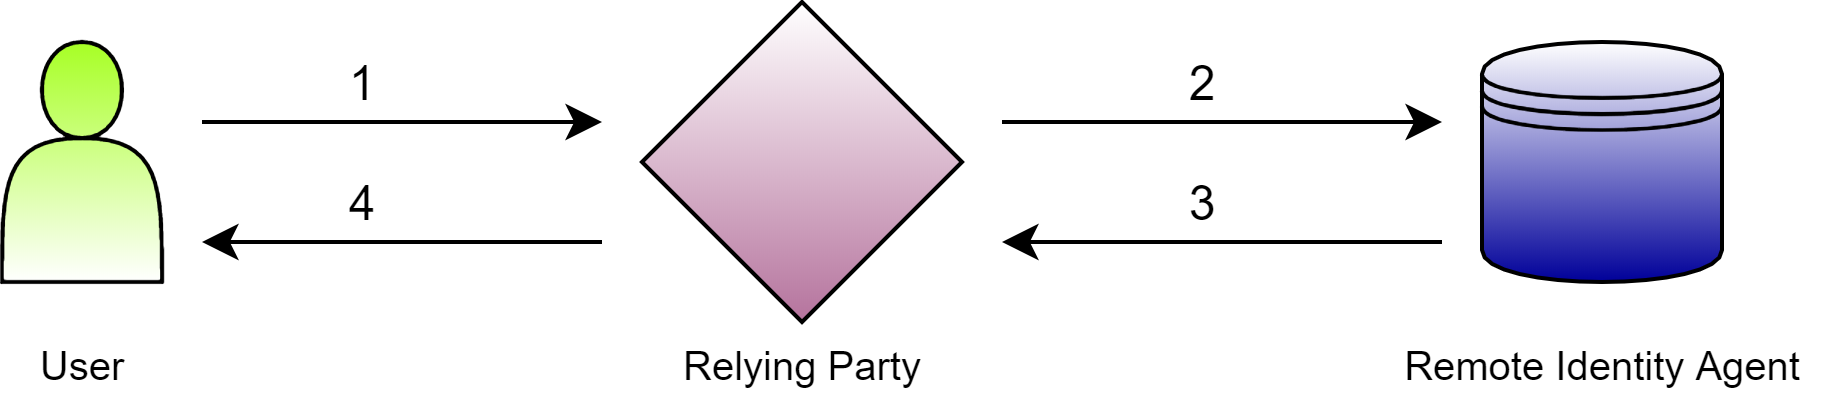
\includegraphics[scale=1]{3.png}
    \caption{Entities}
    \label{fig:threshold}
  \end{figure}

 \subsection{Attribute Type}

 The attribute type is used to identify the entity. There are three major types[11].

 \subsubsection{Who you are}
 In the real world, it is easy to identify a single entity  It can include knowledge or data that is only known by that entity, unique physical characteristics of that entity, or items that the entity possesses.

 \subsubsection{Context}
 Different constraints on digital identity may be implemented depending on the context. For instance, transferring sensitive information relating to birth certificates over the phone or the internet may be prohibited. level of trust is play a major role here, so the context is used to identify the quantity and type of information needed for providing the trust. For example, in an email context, the amount of identifying information necessarily is usually only two things: a username and a password. 

 \subsubsection{Profile}
 After user is verified the profile data is needed for services. User profiles can include what entities can do, what they have subscribed to, what groups they are members of, their selected services, etc. A user’s profile can change during the course of an interaction with the service provider.

\subsection{Lifecycle}
There are three fundamental steps to creating digital identity[12]: registration, including enrollment and validation; issuance of documents or credentials; and authentication for service delivery or transactions.

\begin{figure}[H]
    \centering
    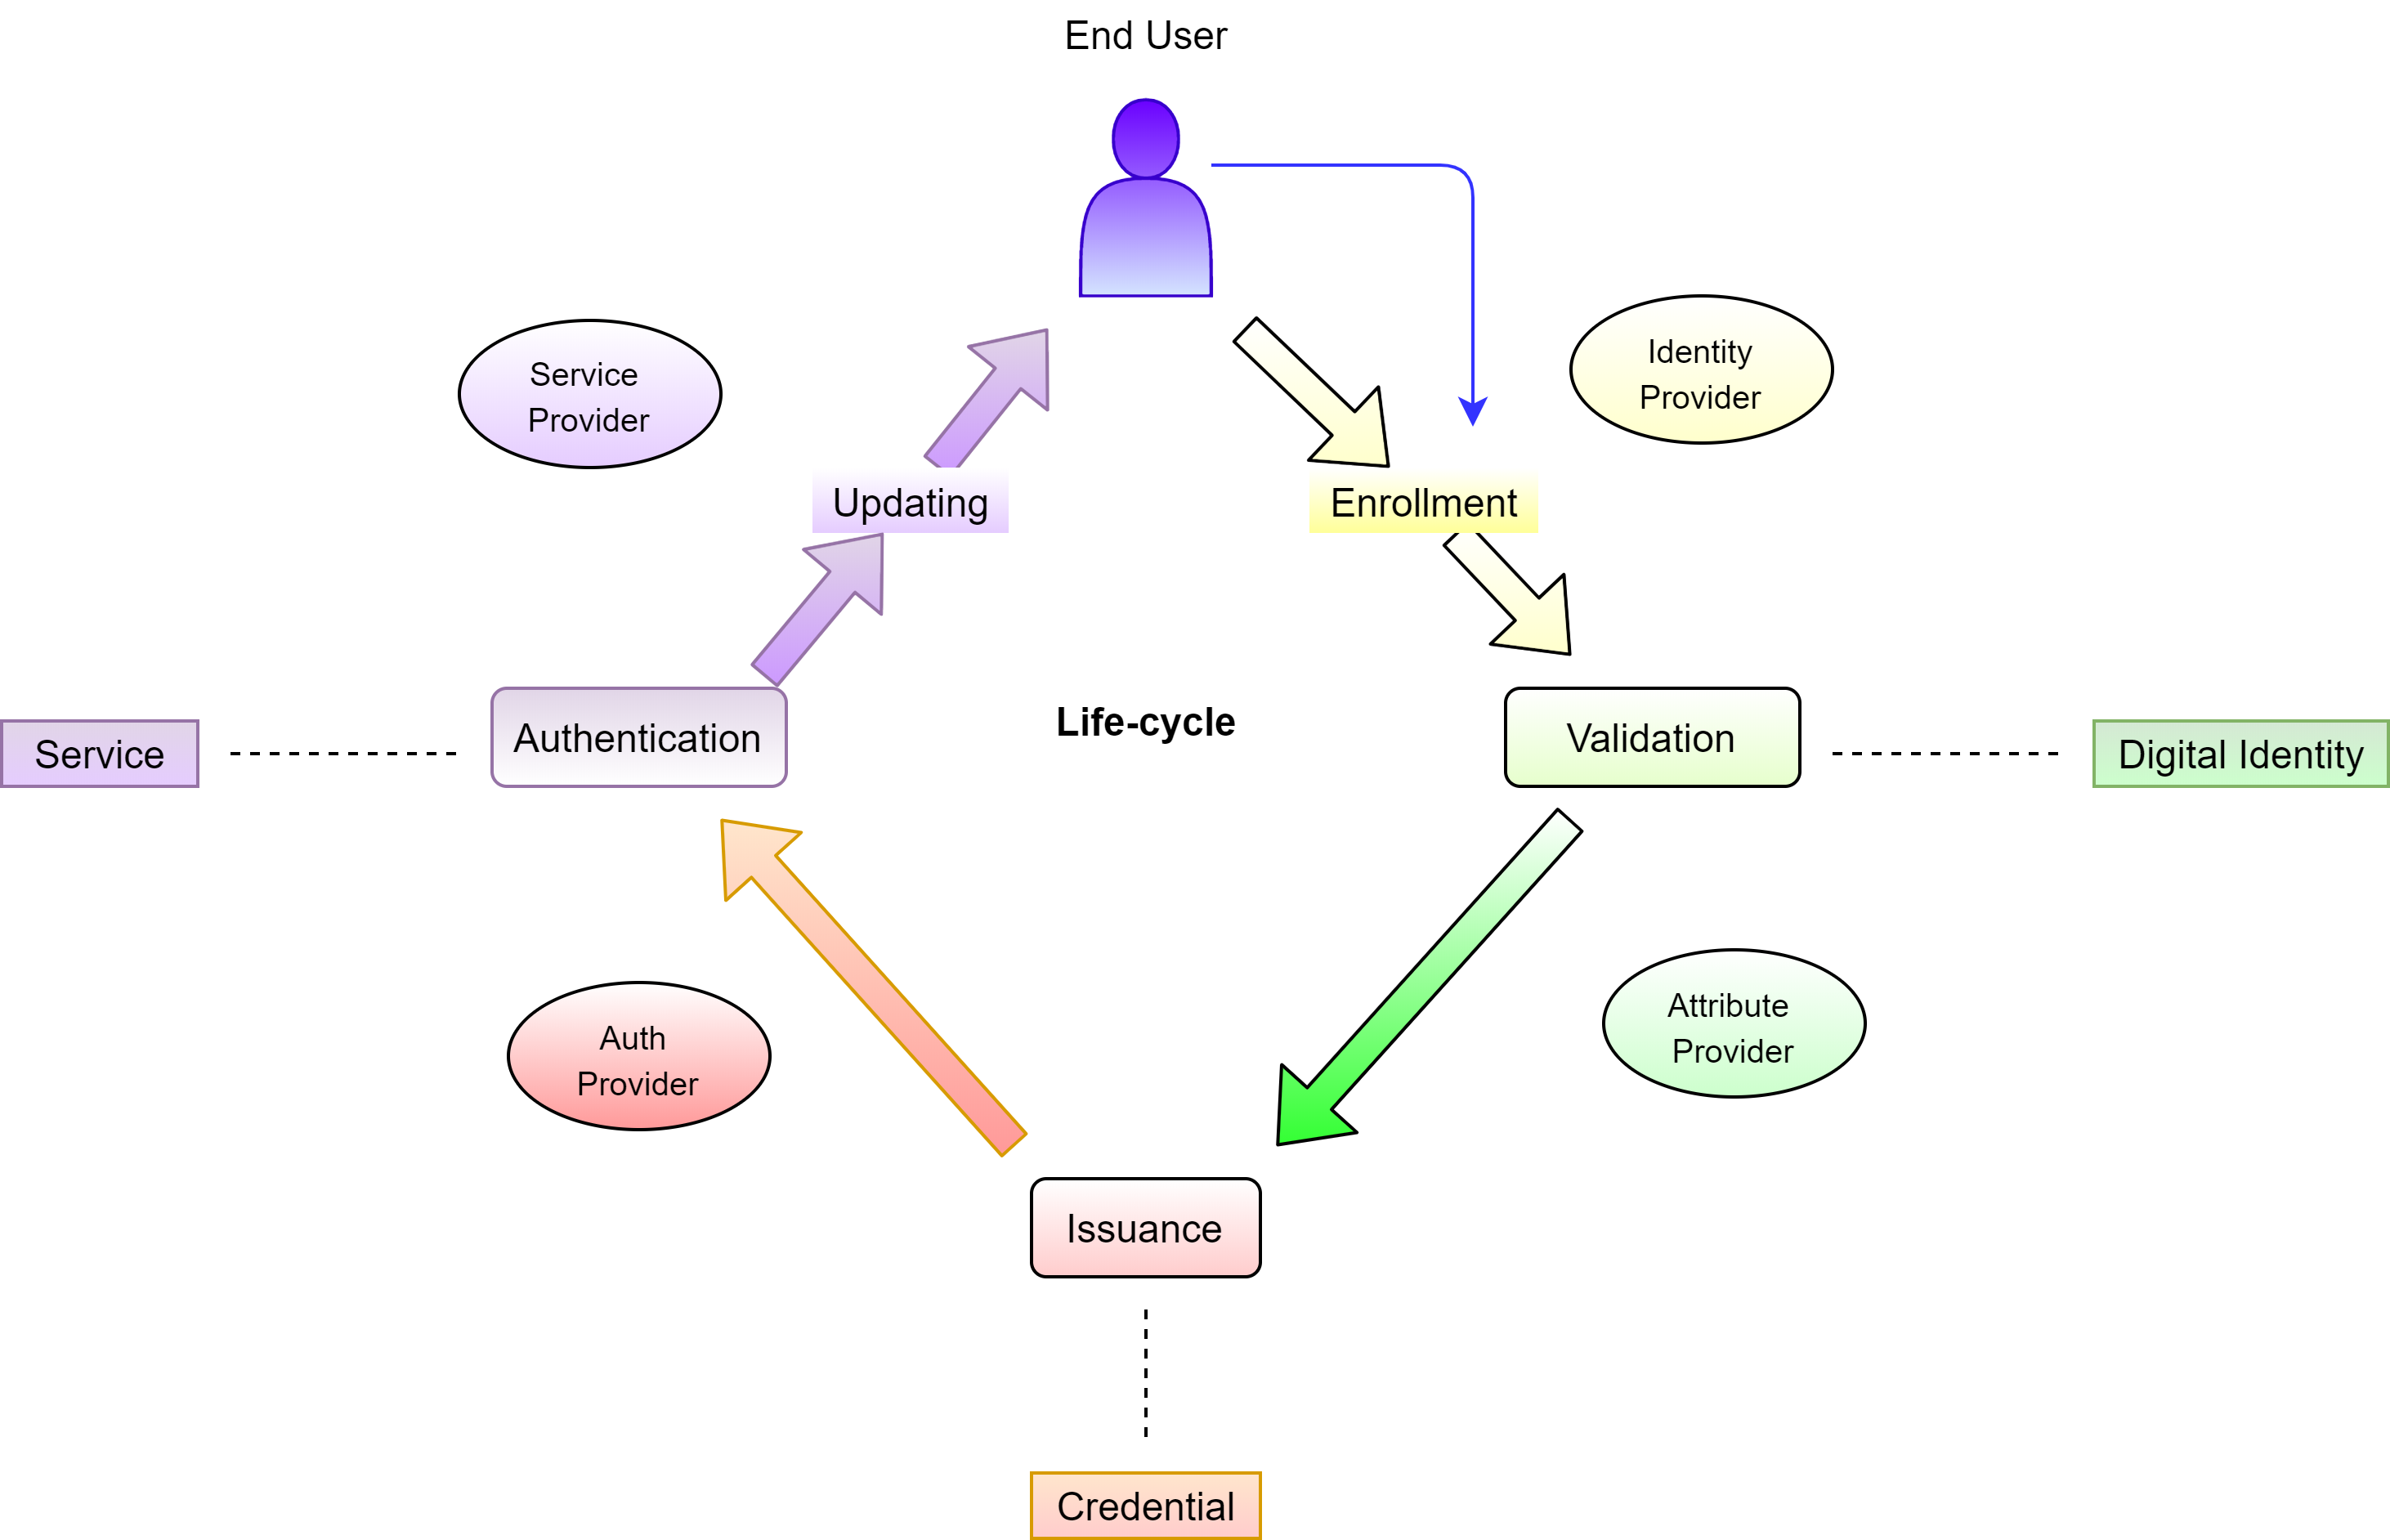
\includegraphics[scale=0.8]{4.png}
    \caption{Digital Identity Lifecycle}
    \label{fig:threshold}
  \end{figure}

  \subsubsection{Enrollment}
  There are two main categories, which are enrollment and validation. Enrollment registration steps: capturing and recording key identity attributes of a person who claims a certain identity. This may include biographical data (e.g., name, date of birth, gender, address, email), biometrics (e.g., fingerprints, iris scan), and the other attributes. 
  
  \subsubsection{Issuance}
  Before it can be used by a person, a registered identity goes through an issuance or credentialing process. For an identity to be considered digital, the credentials or certificates (e.g., birth certificate, passport) issued must be electronic, in the sense that they store and communicate data electronically. Types of electronic credentials including smartcards, 2D barcode cards, mobile identity, and identity in the cloud.

  \subsection{Policies}
  The level of access is conditioned not only by the identity but is also likely constrained by a number of further security considerations, such as the company policy.
  
  \subsection{Technology}
  \subsubsection{Authentication Techniques}
  The authentication processors were varying from different factors. the list of major methods are listed below

  \begin{itemize}
      \item Password or personal identification number (PIN)
  \end{itemize}

  This advanced method involves hashing and the techniques and data are then exchanged with the server and stored [10]. The PIN technique basically has the same mechanism as a password, but it consists of a numeric term only (usually with four to six digits). still, in the world, the pin-based process is following in banks and other business industries. 

  \begin{itemize}
    \item Token
\end{itemize}
  
This works using the two-factor authentication (2FA) principle. Instead of using a username and password, a level is added on to obtain a time-limited token (typically a cryptographic key or password) that is used for further transactions during the session. The physical device for tokens mostly does not require an internet connection because it communicates using mobile telecommunication service operator services such as voice calls, SMS, or USSD. 

\begin{itemize}
    \item Public key cryptography
\end{itemize}

This method utilizes cryptographic mechanisms that, as their underlying theory, engage an asymmetric key pair: a public key and a private key [13]. using the key pair, data encryption and decryption can be done as well as the signing the data can be done using these key pairs.

\begin{figure}[H]
    \centering
    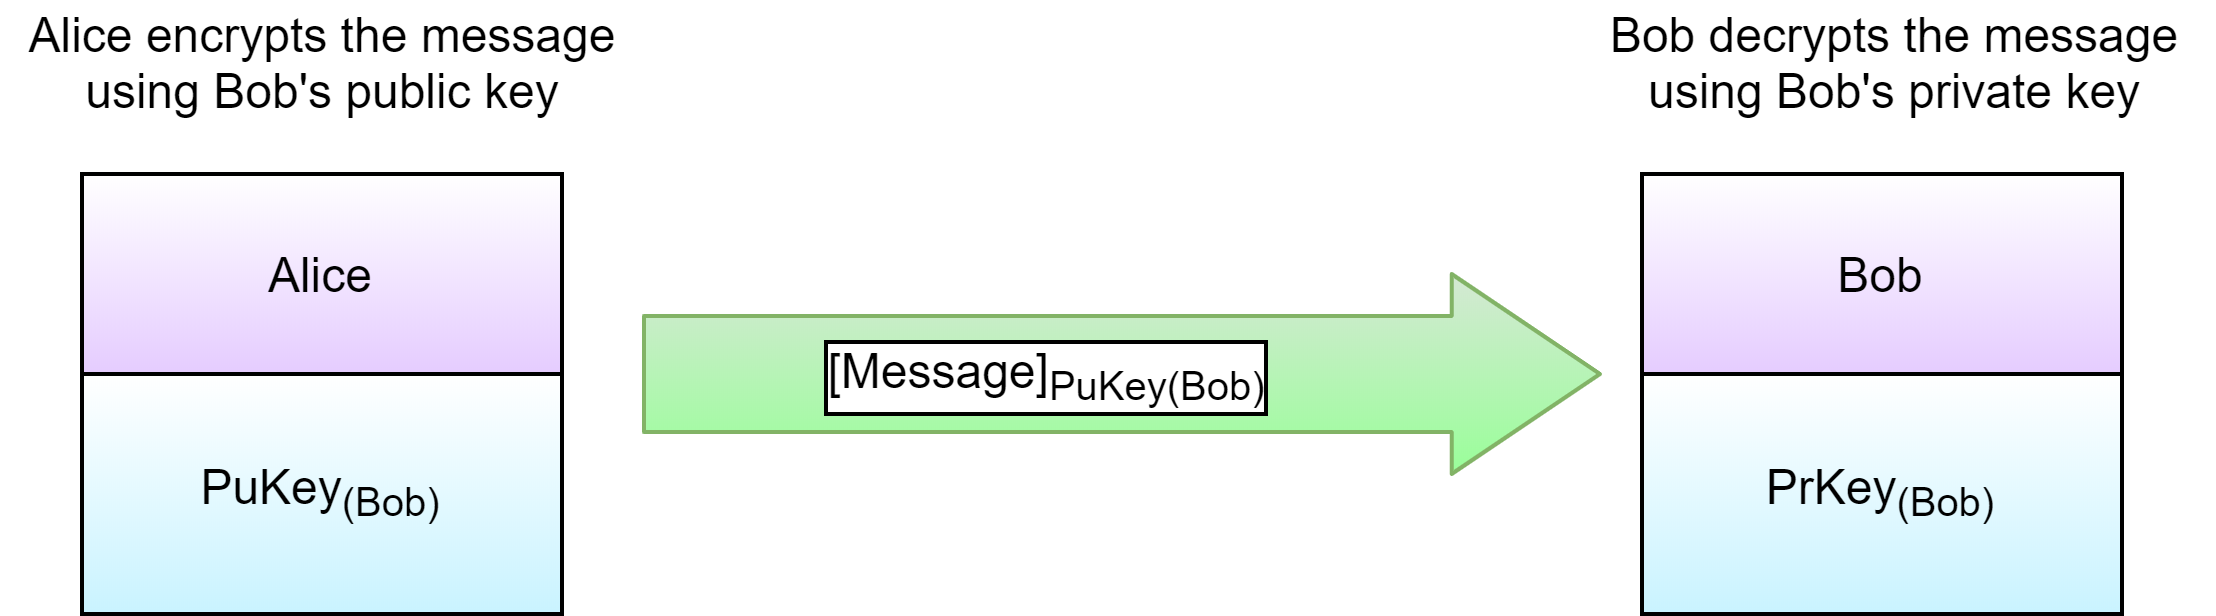
\includegraphics[scale=0.8]{5.png}
    \caption{Keypair cryptography}
    \label{fig:threshold}
  \end{figure}

  \begin{itemize}
    \item Biometric
\end{itemize}

Biometric authentication requires a completely different style of the authentication process. This approach is based on a person’s biological uniqueness and it can be used for the biometric identification of a person [14], using, for example, fingerprint or iris recognition.most of the pattern matching techniques used for this. Biometrics also depends on the devices that are collect data.

\begin{itemize}
    \item Smart Card
\end{itemize}

When used for logical access, smart card technology typically comes in two forms: a credit-card-sized plastic card or a USB device, each with an embedded computer chip [15]. the major application of a smart card is storing a password.

\subsubsection{Security Protocols}

security protocols highly valued because verification and authentications are depended on that. The widespread authentication protocols used to address security issues within open networks are Secure Sockets Layer (SSL), IP Sec, Secure Shell (SSH), and Kerberos [16]. 

\subsubsection{Storage}

There are two new technologies that may offer improved methods in database storage [9]. The first is distributed ledger technology or blockchain combined with encryption and cloud storage, and this allows information to be held and transferred point-to-point in a dispersed, immutable network. The second consists of federated identity standards, such as SAML 2.0, which create interoperability between identity management networks and external applications, allowing federated identity systems to scale to accommodate large numbers of identity providers and relying parties.

single-sign-on (SSO) authentication. plays a major role in the authentication context in this era. This system allows users to sign on only once and have their identities automatically verified by each application or service they want to access afterward[17]. This system serves different purposes[18]. It communicates between applications and the network, it enables communication to applications that are connected by the internet using web resources, and it integrates different domains with different sets of credentials located all over the world. The aim of using SSO is to improve the communication and security of user authentication and access permission verification and also to decrease management costs [19]. Popular examples of SSO systems are found at Google, Microsoft, Facebook, and Yahoo; they provide SSO to their users when accessing emails, groups, documents, and other facilities embedded in their SSO system



  

  


\chapter{Design}
Digital Identity Management is not a replacement discovery within the Information Technology world. Since Ancient Roman times, Passwords have been the ultimate keepers of diversity and
security[5]. Even today, they are used to prove one’s worth for obtaining some privilege others do not possess, but strongly desire to get. However, over the years with the emergence of the web, Identity Management has transformed through several phases, although maintaining the same goals of,

\begin{enumerate}
    \item Authentication - Verifying that an individual is who they claim to be.
    \item Authorization - Providing them access to some associated resources or services.
\end{enumerate}

These two goals, authentication, and authorization are the backbone of access control[6] and work together to get the specified trust necessary to supply resources or services to assumed unknown persons. 

\section{The Concept and Properties of Digital Identity}

The identity concept can be seen from different perspectives and is applicable in different domains, depending on the objective for which digital identity is used. In general, personal identity in philosophy refers to the answer to the question, ‘Who am I?’ It consists roughly of those properties that make the individual unique and different from others[7]. Precisely, identity refers to a set of qualities and characteristics that make an entity definable, distinguishable, and recognizable compared to other entities[8]. However, in the digital world, “identity” is a set of digital records that represents a user. These records are saved and managed in a standard format by entities that provide the identity information or assurances needed to complete transactions. Digital identity also accepts and integrates new records to create a rich view of the user[9]. The following are five properties that should be applied to contribute to a more detailed and provisioning solution of a digital identity system.

\subsection{Entities}

According to its definition, an entity is an object that exists or has its own independent existence. Entity conduct as representation from a unit that bears the legal rights for the system, e.g., individuals, businesses, and affiliates. Those entities can be specifically categorized into three types[10]. They have their own private and public keys and can be run by parties that have certain user credentials, such as banks, universities, or other entities that are trusted by the user. The last type consists of Relying parties, which represent a party with which a user intends to interact, essentially, an online service provider; however, in a peer-to-peer system, relying parties can be other users.

\begin{figure}[H]
    \centering
    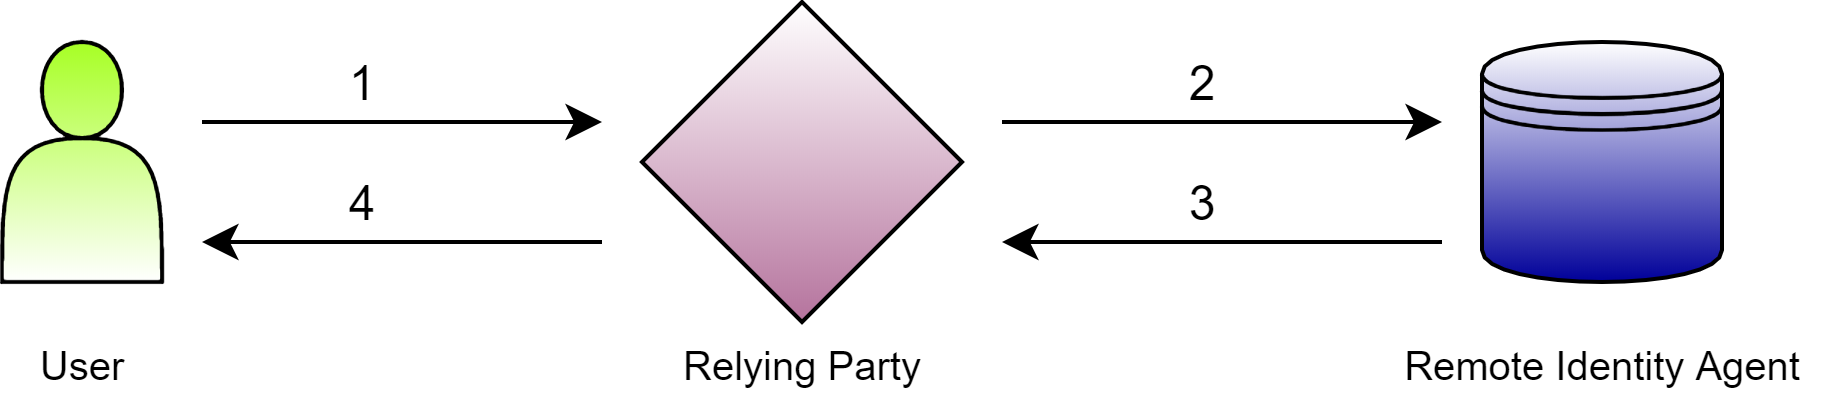
\includegraphics[scale=1]{3.png}
    \caption{Entities}
    \label{fig:threshold}
  \end{figure}

 \subsection{Attribute Type}

 The attribute type is used to identify the entity. There are three major types[11].

 \subsubsection{Who you are}
 In the real world, it is easy to identify a single entity  It can include knowledge or data that is only known by that entity, unique physical characteristics of that entity, or items that the entity possesses.

 \subsubsection{Context}
 Different constraints on digital identity may be implemented depending on the context. For instance, transferring sensitive information relating to birth certificates over the phone or the internet may be prohibited. level of trust is play a major role here, so the context is used to identify the quantity and type of information needed for providing the trust. For example, in an email context, the amount of identifying information necessarily is usually only two things: a username and a password. 

 \subsubsection{Profile}
 After user is verified the profile data is needed for services. User profiles can include what entities can do, what they have subscribed to, what groups they are members of, their selected services, etc. A user’s profile can change during the course of an interaction with the service provider.

\subsection{Lifecycle}
There are three fundamental steps to creating digital identity[12]: registration, including enrollment and validation; issuance of documents or credentials; and authentication for service delivery or transactions.

\begin{figure}[H]
    \centering
    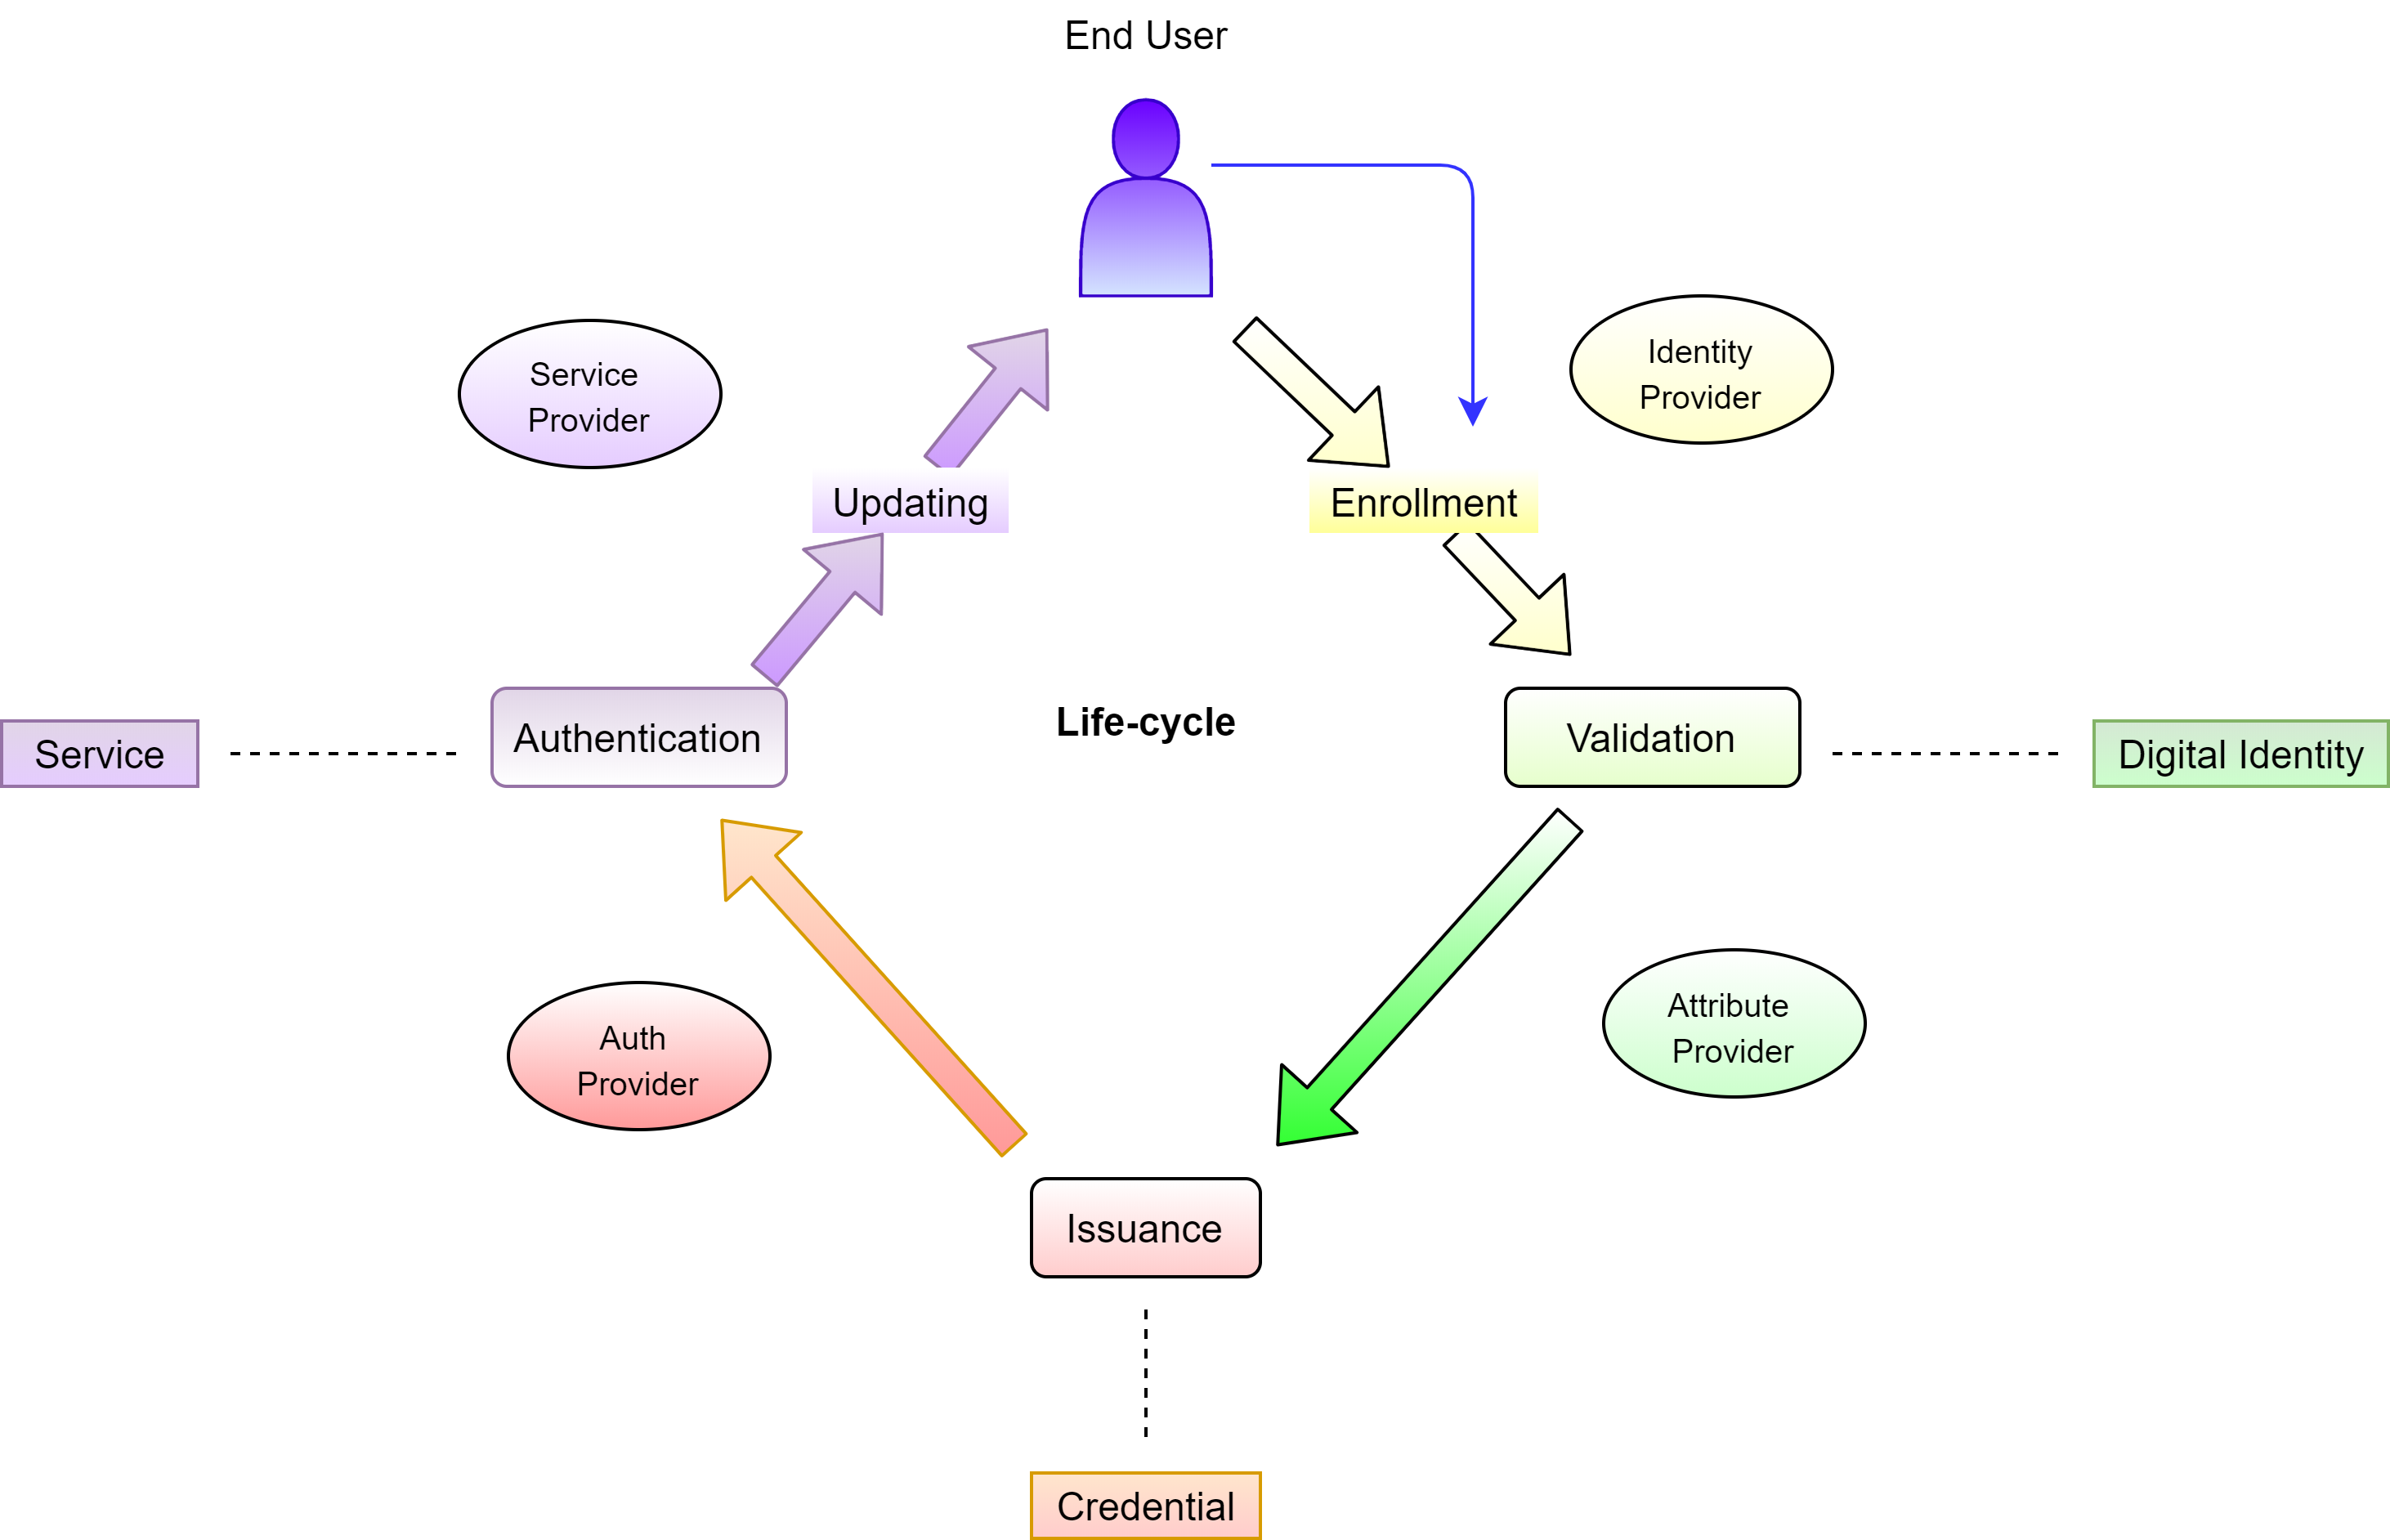
\includegraphics[scale=0.8]{4.png}
    \caption{Digital Identity Lifecycle}
    \label{fig:threshold}
  \end{figure}

  \subsubsection{Enrollment}
  There are two main categories, which are enrollment and validation. Enrollment registration steps: capturing and recording key identity attributes of a person who claims a certain identity. This may include biographical data (e.g., name, date of birth, gender, address, email), biometrics (e.g., fingerprints, iris scan), and the other attributes. 
  
  \subsubsection{Issuance}
  Before it can be used by a person, a registered identity goes through an issuance or credentialing process. For an identity to be considered digital, the credentials or certificates (e.g., birth certificate, passport) issued must be electronic, in the sense that they store and communicate data electronically. Types of electronic credentials including smartcards, 2D barcode cards, mobile identity, and identity in the cloud.

  \subsection{Policies}
  The level of access is conditioned not only by the identity but is also likely constrained by a number of further security considerations, such as the company policy.
  
  \subsection{Technology}
  \subsubsection{Authentication Techniques}
  The authentication processors were varying from different factors. the list of major methods are listed below

  \begin{itemize}
      \item Password or personal identification number (PIN)
  \end{itemize}

  This advanced method involves hashing and the techniques and data are then exchanged with the server and stored [10]. The PIN technique basically has the same mechanism as a password, but it consists of a numeric term only (usually with four to six digits). still, in the world, the pin-based process is following in banks and other business industries. 

  \begin{itemize}
    \item Token
\end{itemize}
  
This works using the two-factor authentication (2FA) principle. Instead of using a username and password, a level is added on to obtain a time-limited token (typically a cryptographic key or password) that is used for further transactions during the session. The physical device for tokens mostly does not require an internet connection because it communicates using mobile telecommunication service operator services such as voice calls, SMS, or USSD. 

\begin{itemize}
    \item Public key cryptography
\end{itemize}

This method utilizes cryptographic mechanisms that, as their underlying theory, engage an asymmetric key pair: a public key and a private key [13]. using the key pair, data encryption and decryption can be done as well as the signing the data can be done using these key pairs.

\begin{figure}[H]
    \centering
    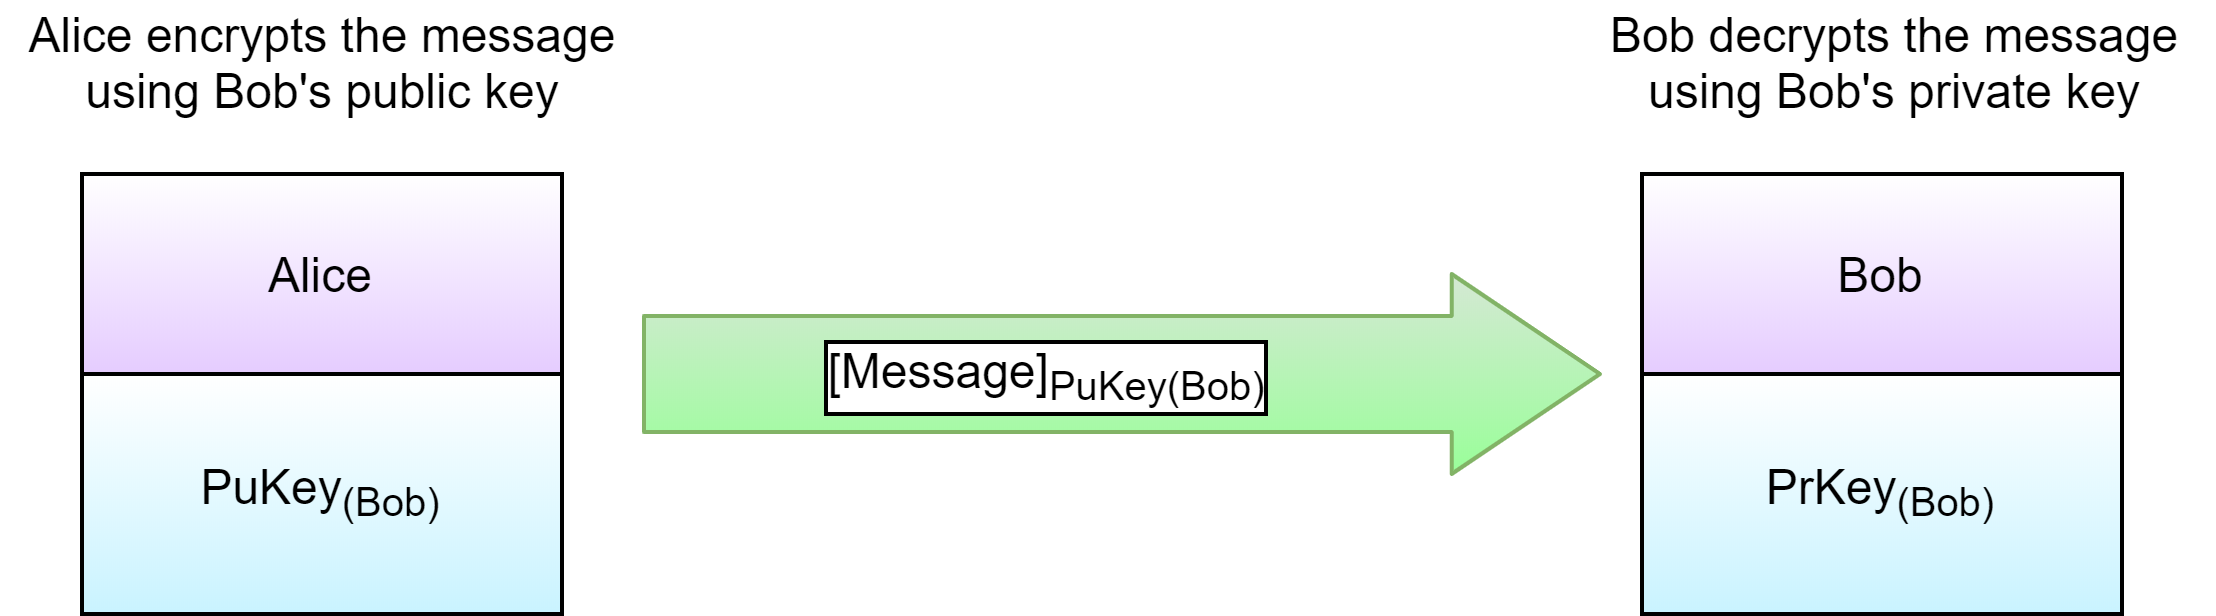
\includegraphics[scale=0.8]{5.png}
    \caption{Keypair cryptography}
    \label{fig:threshold}
  \end{figure}

  \begin{itemize}
    \item Biometric
\end{itemize}

Biometric authentication requires a completely different style of the authentication process. This approach is based on a person’s biological uniqueness and it can be used for the biometric identification of a person [14], using, for example, fingerprint or iris recognition.most of the pattern matching techniques used for this. Biometrics also depends on the devices that are collect data.

\begin{itemize}
    \item Smart Card
\end{itemize}

When used for logical access, smart card technology typically comes in two forms: a credit-card-sized plastic card or a USB device, each with an embedded computer chip [15]. the major application of a smart card is storing a password.

\subsubsection{Security Protocols}

security protocols highly valued because verification and authentications are depended on that. The widespread authentication protocols used to address security issues within open networks are Secure Sockets Layer (SSL), IP Sec, Secure Shell (SSH), and Kerberos [16]. 

\subsubsection{Storage}

There are two new technologies that may offer improved methods in database storage [9]. The first is distributed ledger technology or blockchain combined with encryption and cloud storage, and this allows information to be held and transferred point-to-point in a dispersed, immutable network. The second consists of federated identity standards, such as SAML 2.0, which create interoperability between identity management networks and external applications, allowing federated identity systems to scale to accommodate large numbers of identity providers and relying parties.

single-sign-on (SSO) authentication. plays a major role in the authentication context in this era. This system allows users to sign on only once and have their identities automatically verified by each application or service they want to access afterward[17]. This system serves different purposes[18]. It communicates between applications and the network, it enables communication to applications that are connected by the internet using web resources, and it integrates different domains with different sets of credentials located all over the world. The aim of using SSO is to improve the communication and security of user authentication and access permission verification and also to decrease management costs [19]. Popular examples of SSO systems are found at Google, Microsoft, Facebook, and Yahoo; they provide SSO to their users when accessing emails, groups, documents, and other facilities embedded in their SSO system



  

  


\chapter{Implementation}
\paragraph{}
This chapter elaborates the implementation details of the proposed design. 

\section{Indy framework}
Indy is a subproject of hyperledger project. It is designed and developed by the Linux Foundation. Hyperledger project has several sub-projects for different use cases. Indy is developed for the Identity Management use case. For all these reasons, the Indy Project has developed specifications, terminology, and design patterns for decentralized identity along with an implementation of these concepts that can be leveraged and consumed both inside and outside the Hyperledger Project. This framework allows to build a normal blockchain(a public blockchain). The research design should be implemented on top of that. In order to that, the first step is to dockerize the environment. The following implementations are going on top of that a docker image which has a couple of nodes as docker containers. 

\paragraph{}
The implementation is running on Jupyter notebook as python environment and codebase is written in python.

\section{Configure the pool}
Nodes are located in the node pool which is the network. Every node has a different IP address and networking every one of them makes the node pool. Those nodes are stored inside the pool ledger(node transactions). This is the place where blockchain sets up its genesis transaction path. 

\begin{verbatim}
    await pool.set_protocol_version(2)

    pool_ = {
        'name': 'pool1',
        'config': json.dumps({"genesis_txn": '/home/indy/sandbox/pool_transactions_genesis'})
    }
    print("Open Pool Ledger: {}".format(pool_['name']))

    try:
        await pool.create_pool_ledger_config(pool_['name'], pool_['config'])
    except IndyError as ex:
        if ex.error_code == ErrorCode.PoolLedgerConfigAlreadyExistsError:
            pass
    pool_['handle'] = await pool.open_pool_ledger(pool_['name'], None)

\end{verbatim}

\section{Setting up Steward Role}

\paragraph{}
Steward is the one who created the chain and genesis block are defined by this role. It creates the NYM transaction(creation of a DID in the ledger) and created a wallet. Indy has this concept called a wallet that is secure storage for DIDs, keys and other crypto materials. The steward’s wallet is created and store the did. Then steward can obtain trust anchor role.

\begin{verbatim}
    steward = {
        'name': "Sovrin Steward",
        'wallet_config': json.dumps({'id': 'sovrin_steward_wallet'}),
        'wallet_credentials': json.dumps({'key': 'steward_wallet_key'}),
        'pool': pool_['handle'],
        'seed': '000000000000000000000000Steward1'
    }

    await create_wallet(steward)

    print("\"Sovrin Steward\" -> Create and store in Wallet DID from seed")
    steward['did_info'] = json.dumps({'seed': steward['seed']})
    steward['did'], steward['key'] = await did.create_and_store_my_did(steward['wallet'], steward['did_info’]
\end{verbatim}

\paragraph{}
These DIDs are using base58Check encoding.

\section{Obtaining verinym for organizations}

\paragraph{}
Every identity owner has a legal identity. A verinym is a DID which related to this legal identity. In order to join the chain organizations should create this verinym. It happens in a couple of steps.

\begin{enumerate}
    \item Creates a wallet if the organization is new to the chain\\
    Birth certificates are issued by the Registrar General’s Department(RGD). This RGD would be the first organization that register with this chain. 
    \begin{verbatim}
        await wallet.create_wallet(rgd['wallet_config'], rgd['wallet_credentials'])
        rgd['wallet'] = await wallet.open_wallet(rgd['wallet_config'], rgd['wallet_credentials'])
    \end{verbatim}

    \item Create a DID in the wallet.
    \begin{verbatim}
        # RGD Agent
        (rgd['did'], rgd['key']) = await did.create_and_store_my_did(rgd['wallet'], "{}")
    \end{verbatim}

    \item Registrar General’s Department creates a message with DID and key.
    \begin{verbatim}
        # RGD Agent
        rgd['did_info'] = json.dumps({
            'did': rgd['did'],
            'verkey': rgd['key']
        })
    \end{verbatim}

    \item Send the DID info message to Steward. This is how a communication channel is created.
    \begin{verbatim}
        steward['rgd_info'] = rgd['did_info'] 
    \end{verbatim}

    \item Steward is a trust anchor, so he can send the transaction to the ledger(NYM transaction). But the DID owner is RDG.
    \begin{verbatim}
        # Steward Agent
        nym_request = await ledger.build_nym_request(steward['did'], steward['rgd_info']['did'],
                                                    steward['rgd_info']['verkey'], None, 'TRUST_ANCHOR')
        await ledger.sign_and_submit_request(steward['pool'], steward['wallet'], steward['did'], nym_request)
    \end{verbatim}
\end{enumerate}

\paragraph{}
After this step, RGD has a DID from his identity in the ledger. The every other organization should do the same in order to create a DID. The government is also an organization registered in the chain.

\section{Schemas Setup for credentials}

\paragraph{}
Schemas are structures that consist of attributes names and details of a credential. Credentials cannot be altered, that is why it maintains a version number. The government is a trust anchor which already created. Every trust anchor can publish credential schema to the ledger.

\paragraph{}
Schema for Birth certificate

\begin{verbatim}
    {
      'name': 'Birth Certificate',
      'version': '1.0',
      'attributes': ['first_name', 'last_name', '', 'birth_date', ‘sex’, ‘Address, ‘Registrar’s_devision’’,’father_name’,’mother_name’,’certificate_number’]
    }
\end{verbatim}

\begin{enumerate}
    \item Create the schema 
    \begin{verbatim}
        # Government Agent
        birth_certificate = {
            'name': 'Birth Certificate',
            'version': '1.0',
            'attributes': ['first_name', 'last_name', '',
                        'birth_date', ‘sex’, ‘Address, ‘Registrar’s_devision’’, ’father_name’, ’mother_name’, ’certificate_number’]
        }

        (government['birth_certificate_schema_id'], government['birth_certificate_schema']) = \
            await anoncreds.issuer_create_schema(government['did'], birth_certificate['name'], birth_certificate['version'],
                                                json.dumps(birth_certificate['attributes']))
        birth_certificate_schema_id = government['birth_certificate_schema_id']
    \end{verbatim}

    \item The government (trust anchor) sends the schema to the ledger.
    \begin{verbatim}
        # Government Agent
        schema_request = await ledger.build_schema_request(government['did'], government['transcript_schema'])
        await ledger.sign_and_submit_request(government['pool'], government['wallet'], government['did'], schema_request)
    \end{verbatim}
\end{enumerate}

\section{Setup of credential definition}

\paragraph{}
Issuer signs the credentials here.

\begin{enumerate}
    \item RDA gets the credential schema.
    \begin{verbatim}
        # RGD Agent
        get_schema_request = await ledger.build_get_schema_request(rgd['did'], birth_certificate_schema_id)
        get_schema_response = await ledger.submit_request(rgd['pool'], get_schema_request) 
        rgd['birth_certificate_schema_id'], rgd['birth_certificate_schema'] = await ledger.parse_get_schema_response(get_schema_response)
    \end{verbatim}

    \item Create a credential definition. Then it stores in the wallet of RGD(cannot read)
    \begin{verbatim}
        # RGD Agent
        birth_certificate_cred_def = {
            'tag': 'TAG1',
            'type': 'CL',
            'config': {"support_revocation": False}
        }
        (rgd['birth_certificate_cred_def_id'], rgd['birth_certificate_cred_def']) = \
            await anoncreds.issuer_create_and_store_credential_def(rgd['wallet'], rgd['did'],
                                                                rgd['birth_certificate_schema'], birth_certificate_cred_def['tag'],
                                                                birth_certificate_cred_def['type'],
                                                                json.dumps(birth_certificate_cred_def['config']))
    \end{verbatim}

    \item Update the ledger by sending the credential definition. It is done by the trust anchor(RGD).
    \begin{verbatim}
        # RGD Agent     
        cred_def_request = await ledger.build_cred_def_request(rgd['did'], rgd['birth_certificate_cred_def'])
        await ledger.sign_and_submit_request(rgd['pool'], rgd['wallet'], rgd['did'], cred_def_request)
    \end{verbatim}
\end{enumerate}

\section{The user gets a credential (a birth certificate)}

\paragraph{}
There is a user with no credentials initially. This is how the user gets credentials. A user called “Pasindu” gets a birth certificate from the Registrar General’s Department.

\begin{verbatim}
    # RGD Agent
    rgd['birth_certificate_cred_offer'] = await anoncreds.issuer_create_credential_offer(rgd['wallet'], rgd['birth_certificate_cred_def_id'])
    
    pasindu['birth_certificate_cred_offer'] = rgd['birth_certificate_cred_offer']
\end{verbatim}

\paragraph{}
This birth certificate is issued by the RGD.
Then the user needs a master key to the wallet

\begin{verbatim}
    # Pasindu Agent
  pasindu['master_secret_id'] = await anoncreds.prover_create_master_secret(pasindu['wallet'], None)
\end{verbatim}

\paragraph{}
In order to make a credential request, the user needs to credential definition.

\begin{verbatim}
    # Pasindu Agent
    get_cred_def_request = await ledger.build_get_cred_def_request(pasindu['did_for_rgd'], pasindu['birth_certificate_cred_offer']['cred_def_id'])
    get_cred_def_response = await ledger.submit_request(pasindu['pool'], get_cred_def_request)
    pasindu['birth_certificate_cred_def'] = await ledger.parse_get_cred_def_response(get_cred_def_response)
\end{verbatim}

\paragraph{}
Now, the user can request the credentials

\begin{verbatim}
    # Pasindu Agent
    (pasindu['birth_certificate_cred_request'], pasindu['birth_certificate_cred_request_metadata']) = \
        await anoncreds.prover_create_credential_req(pasindu['wallet'], pasindu['did_for_rgd'], pasindu['birth_certificate_cred_offer'],
                                                     pasindu['birth_certificate_cred_def'], pasindu['master_secret_id'])
                                                     
    rgd['birth_certificate_cred_request'] = pasindu['birth_certificate_cred_request']

\end{verbatim}

\paragraph{}
The organization(RGD) creates the schema with raw and encoded values.

\begin{verbatim}
    # RGD Agent
    # note that encoding is not standardized by Indy except that 32-bit integers are encoded as themselves. IS-786
    birth_certificate_cred_values = json.dumps({
        "first_name": {"raw": "Pasindu", "encoded": "1139481716457488690172217916278103335"},
        "last_name": {"raw": "Lakshitha", "encoded": "5321642780241790123587902456789123452"},
        "birth_date": {"raw": "1995.09.25", "encoded": "12434523576212321"},
        "sex": {"raw": "male", "encoded": "2213454313412354"},
        "Address": {"raw": "76,Biyagama RD,Kelaniya", "encoded": "3124141231422543541"},
        "Registrar’s_devision": {"raw": "Gampaha", "encoded": "2015"},
        "father_name": {"raw": "K.A. Perera", "encoded": "2414123142254354"},
    "mother_name": {"raw": "M.L. Wickramsinghe", "encoded": "14123142"},
    "certificate_number": {"raw": "231131", "encoded": "4545454313412354"},


    })
    rgd['birth_certificate_cred'], _, _ = \
        await anoncreds.issuer_create_credential(rgd['wallet'], rgd['birth_certificate_cred_offer'], rgd['transcript_cred_request'],
                                                birth_certificate_cred_values, None, None)
                                                
    pasindu['birth_certificate_cred'] = rgd['birth_certificate_cred']
\end{verbatim}

\paragraph{}
Now, credentials for a birth certificate(credential) has been issued by the RGD(issuer/organization). and Pasindu(User) can store the credentials in his wallet.

\begin{verbatim}
    # Pasindu Agent
    await anoncreds.prover_store_credential(pasindu['wallet'], None, rgd['birth_certificate_cred_request'], rgd['birth_certificate_cred_request_metadata'],
                                            pasindu['birth_certificate_cred'], pasindu['birth_certificate_cred_def'], None)

\end{verbatim}

\section{How to use the credentials}

\paragraph{}
Now user has his credentials stores in the wallet. There is another organization that is in the chain called the Department of Motor Traffic(DMT/RMV) like RGD. after established the connection between the user(Pasindu) and the organization(RMV), the user got the license application proof request in order to apply for a driving license.

\begin{verbatim}
    # RMV Agent
    rmv['application_proof_request'] = json.dumps({
        'nonce': '1432422343242122312411212',
        'name': 'Driving-license-Application',
        'version': '0.1',
        'requested_attributes': {
            'attr1_referent': {
                'name': 'first_name'
            },
            'attr2_referent': {
                'name': 'last_name'
            },
            'attr3_referent': {
                'name': 'sex',
                'restrictions': [{'cred_def_id': rgd['transcript_cred_def_id']}]
            },
            'attr4_referent': {
                'name': 'birth_date',
                'restrictions': [{'cred_def_id': rgd['transcript_cred_def_id']}]
            },
            'attr5_referent': {
                'name': 'address',
                'restrictions': [{'cred_def_id': rgd['transcript_cred_def_id']}]
            },
            'attr6_referent': {
                'name': 'phone_number'
            }
        }
            })
    
    pasindu['application_proof_request'] = rmv['birth_certificate_cred']
\end{verbatim}

\paragraph{}
The proof request asks to sex, address, birth\_date in the credentials should be asserted by an issuer and the key of the schema. Only several attributes can be verifiable in the above proof request.

\paragraph{}
The user(Pasindu ) has only one credential to prove the requirements in his wallet. In order to fill the application, Pasindu can decide what attributes should be revealed.

\begin{verbatim}
    #Pasindu Agent
    pasindu['application_requested_creds'] = json.dumps({
        'self_attested_attributes': {
            'attr1_referent': 'Pasindu',
            'attr2_referent': 'Lakshitha',
            'attr6_referent': '123-45-6789'
        },
        'requested_attributes': {
            'attr3_referent': {'cred_id': cred_for_attr3['referent'], 'revealed': True},
            'attr4_referent': {'cred_id': cred_for_attr4['referent'], 'revealed': True},
            'attr5_referent': {'cred_id': cred_for_attr5['referent'], 'revealed': True},
        },
        'requested_predicates': {'predicate1_referent': {'cred_id': cred_for_predicate1['referent']}}
    })

\end{verbatim}

\paragraph{}
The user needs to reveal only 3 attributes(sex,birth\_date, address). then the user can make a proof request for the application.

\begin{verbatim}
    # Pasindu Agent
    pasindu['apply_license_proof'] = \
            await anoncreds.prover_create_proof(pasindu['wallet'], pasindu['application_proof_request'], pasindu['application_requested_creds'],
                                                pasindu['master_secret_id'], pasindu['schemas'], pasindu['cred_defs'], pasindu['revoc_states'])

    rmv['apply_job_proof'] = pasindu[apply_license_proof]
\end{verbatim}

\paragraph{}
The proof that RMV received is as follows

\begin{verbatim}
    # RMV Agent
    {
        'requested_proof': {
            'revealed_attrs': {
                'attr4_referent': {'sub_proof_index': 0, 'raw':'birth_date', 'encoded':'2213454313412354'},
                'attr5_referent': ['sub_proof_index': 0, 'raw':'sex', 'encoded':'3124141231422543541'},
                'attr3_referent': ['sub_proof_index': 0, 'raw':'address', 'encoded':'12434523576212321'}
            },
            'self_attested_attrs': {
                'attr1_referent': ‘Pasindu',
                'attr2_referent': 'Lakshitha',
                'attr6_referent': '123-45-6789'
            },
            'unrevealed_attrs': {},
            'predicates': {
                'predicate1_referent': {'sub_proof_index': 0}
            }
        },
        'proof' : [] # Validity Proof that RMV can check
        'identifiers' : [ # Identifiers of credentials were used for Proof building
            {
                'schema_id': certificate_schema_id,
                'cred_def_id': rgd_birth_certificate_cred_def_id,
                'rev_reg_id': None,
                'timestamp': None
            }
        }
    }
\end{verbatim}

\paragraph{}
Rmv got all the required details and how it verifies as follows.

\begin{verbatim}
    # RMV Agent
assert await anoncreds.verifier_verify_proof(rmv['application_proof_request'], rmv[apply_license_proof], rmv['schemas'], rmv['cred_defs'], rmv['revoc_ref_defs'], rmv['revoc_regs'])
\end{verbatim}

\paragraph{}
As the final outcome the organization(RMV) can accept the client(register for the driving license).

\begin{verbatim}
    # RMV Agent
    rmv['certificate_cred_offer'] = await anoncreds.issuer_create_credential_offer(rmv['wallet'], rmv['certificate_cred_def_id'])
    
    pasindu['certificate_cred_offer'] = rmv['certificate_cred_offer']
\end{verbatim}

\chapter{Results and Evaluation}

\chapter{Conclusions}


\renewcommand\bibname{References}
\bibliography{references} 
\addcontentsline{toc}{chapter}{References}
\bibliographystyle{ieeetr}

\end{document}

